\section{Definition of Coordination Operators between the TFSM and Activity Language}
\begin{itemize}
	\item In this section, we use \bcool to capture the specification of two coordination patterns between the TFSM and Activity language. We organize the specification around two operators named  \emph{startActivityWhenEnter} and \emph{AtomicActions}. In the following, we present each operator together with the \bcool specification.
	
	\item The \emph{startActivityWhenEnter} operator captures a hierarchical coordination pattern between TFSM and Activity models, unlike hierarchical coordination frameworks where the semantics is hidden, this operator explicitly specifies how the hierarchical coordination is implemented. In our case, we chose the semantics in which entering a specific state of a TFSM model triggers the execution of a given Activity. When leaving a state, several semantic variation points may be chosen. The outgoing transitions from a state can be considered, for instance, as preemptive for the activity model (\ie firing a transition from a state to another preempts the internal activity). Alternatively, the transition can be considered as non-preemptive (\ie the states cannot be left before the associated activity finishes). In Ptolemy~\cite{modalsptolemybib}, such semantics variations are identified by different graphical representations. In our case, we chose non-preemptive transitions and we specify this in a \bcool specification.  
	 
	\item The \emph{startActivityWhenEnter} operator (Listing~\ref{lst:bcoolStartActivityWhenEnter}) coordinates the action of entering into a state with the starting of an activity so that when a state is entered, the execution of the activity is started. Then, the operator expresses that the activity executes in a loop until the state is left. Entering into a state is identified by the \textit{entering} \dse defined in the context of State. Instances of such \dse have to be coordinated with instances of the \textit{startActivity} \dse. Similarly, leaving a state is identified by \dse \textit{leaving} and finishing an activity is identified by \dse \textit{finishActivity}. The operator selects instances of \dse \emph{startActivity} and \emph{finishActivity} by using their context (Listing~\ref{lst:bcoolStartActivityWhenEnter}: line 5). The pairs selected identify the starting and finishing of an activity. Then, we select the activities that represent a state by relying on the method \emph{onEnterAction} that is defined in the context of State. It specifies the name of the activity that the state represents. 
	
	\item To coordinate the selected instances of \dse, we rely on the event relation \emph{LoopFromStartToFinishNonPeemptive} which makes the internal activity to execute in a loop until the state is left. The relation takes four events as parameters: the events \emph{modeEnter} and \emph{modeLeave} that represents respectively the entering and leaving of a state; and the events \emph{startActivity} and \emph{finishActivity} that represents respectively the starting and finishing of an activity. To specify this relation, we base on \moccml and its ability to define state-based relations (see Figure~\ref{fig:looprelation}). The state-based representation is made of two states named \emph{waitEnterState} and \emph{canLoop}. In waitEnterState state, only the event modeEnter can occur. When this event happens, the state \emph{canLoop} is reached and the events startActivity and finishActivity are allowed to occur. Only when the event modeLeave and finishActivivity happens simultaneously, the state can be left and the activity stops to execute. The use of this relation in the coordination rule results in a hierarchical coordination in which the transitions in the TFSM cannot preempt the execution of the internal activities. The entering a state makes the activity to execute in a loop. Then, only after the activity has finished, the state can be left.
	
	\item Similar than the \emph{startActivityWhenEnter} operator, the \emph{AtomicActions} operator also defines a hierarchical coordination between states and activities, but in this case, it deals with the temporal aspects of the coordination. The operator specifies how the time in the TFSM elapses during the execution of the activities that specify the on-entry action of a state. Thus, this coordination is also hierarchical, but in this case, only considers the timing aspects.

	
	
	\item In the TFSM language, each state machine has a \emph{localClock} used to measure the time while the Activity language is untimed. The local clock is a \emph{FSMClock}, which defines a \dse named \emph{ticks} whose occurrences represent a physical time increment. In the Activity language, the duration of activities can be represented as the time between the \dse \emph{startActivity} and \dse \emph{finishActivity}. 
	\item To coordinate the time, it is necessary to specify the number of \emph{ticks} of the local clock between the occurrence of the \dse \emph{startActivity} and \emph{finishActivity}.
	
	\item We propose an operator thet enforces the execution of the ``internal'' activity to be atomic with respect to the time in the TFSM model. As a result, there is no occurrence of the \dse ticks of the corresponding local clock during the execution of the activity.
	
	
	\item The \emph{AtomicActions} operator (Listing~\ref{lst:bcoolStartActivityWhenEnter}: line 11) specifies how time is consumed during the execution of the activities that are represented by states. It selects instances of \dse \emph{startActivity} and \emph{finishActivity} by using their context. As a result, the pairs selected identify the starting and finishing of an activity. Then, we select the activities that represent a state. To do so, we use the onEnterAction. Then, we use the selected instances of \dse entering to select instances of \dse ticks of the corresponding local clock (Listing~\ref{lst:bcoolStartActivityWhenEnter}: line 12). 
	
	\item To express the coordination rule, we rely on the event relation \emph{AtomicExec}. The event relation accepts three events as parameters: \emph{ticks}, \emph{startAct} and \emph{finishAct}. While the event ticks represents the ticking of the local clock, the startAct and finishAct events represent respectively the starting and finishing of an activity. Figure~\ref{fig:atomicexec} illustrates the state-based representation of the event relation that is made of two states named \emph{waitstartActivity} and \emph{waitfinishActivity}. In \emph{waitstartActivity} state, the event ticks is allowed to occur. Then, when the startAct event happens, the \emph{waitfinishActivity} state is reached and the event is forbidden to occurs, \ie the time in the tfsm does not elapse. Only when the event finishAct happens, the \emph{waitstartActivity} state is reached, and \emph{ticks} is allowed to occur again. In the operator, we use this relation to make the execution of the activities atomic, \ie there is no occurrence of the \dse ticks of the corresponding local clock during the execution of the activity.
	
	\item In this section, we used \bcool to define a set of coordination operators that specify a hierarchical coordination between the TFSM and Activities language. We dealt with both the control and timing aspects of the hierarchical coordination. In the following section, we rely on this \bcool specification to coordinate the models of a surveillance camera system.
	   %  The specification also contains the operator defined in the previous section that enables the coordination of Action and FSMEvents by relying in theirs names (It is now shown in Listing). 
\end{itemize}


\begin{lstlisting}[language=bcool,
caption={Timing and Hierarchical operator between TFSM and fUML languages},
label={lst:bcoolStartActivityWhenEnter}, 
basicstyle=\scriptsize\ttfamily, backgroundcolor=\color{LGrey}, numbers=left, xleftmargin=2pt]
BCOoLSpec TFMSandActivityHierarhicalOperators
	ImportLib "facilities.moccml"
	ImportInterface "activitySemantics.ecl" as activity
	ImportInterface "TFSM.ecl" as tfsm

Operator  StartActivityWhenEnter (activityStart : ad::startActivity , activityStop : ad::finishActivity, enterState : tfsm::entering, leaveState : tfsm::leaving)
when ((activityStart.name = activityStop.name ) and (enterState.name = leaveState.name) and (activityStart.name = enterState.onEnterAction.name));
do 
	LoopFromStartToFinishNonPeemptive (enterState, leaveState, activityStart, activityStop)
end operator;

Operator AtomicActions (activityStart : ad::startActivity , activityStop : ad::finishActivity, enterState : tfsm::entering, leaveState : tfsm::leaving, timeTicks : tfsm::ticks)
when ((activityStart.name = activityStop.name ) and (activityStart.name=enterState.OnEnterAction.name ) and (enterState.owningFSM.localClock = timeTicks));
do 
	AtomicExec (activityStart, activityStop, timeTicks)
end operator;
\end{lstlisting}


\begin{figure}[h]
	\centering
	\subfigure[\emph{LoopFromStartToFinishNonPreemptive} event relation]{
		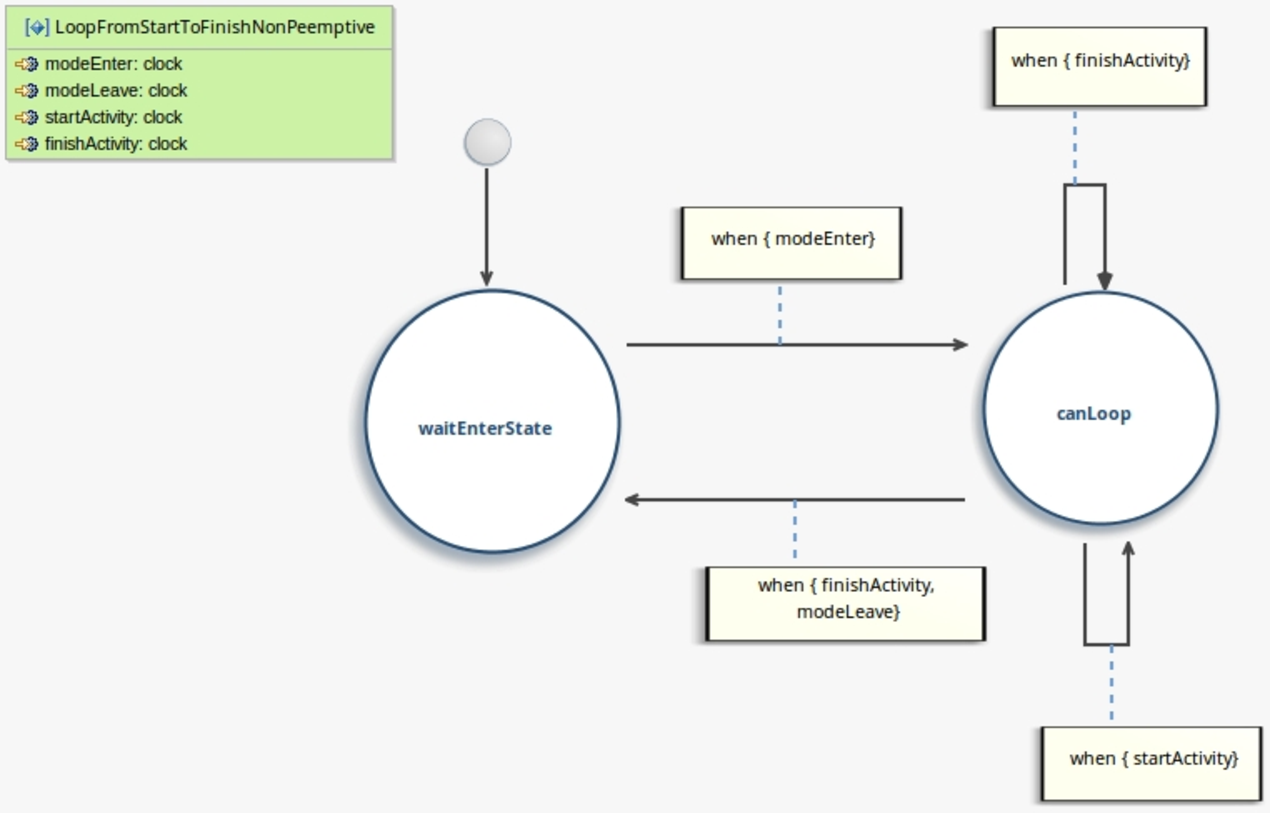
\includegraphics[width=.5\columnwidth]{examples/figs/LoopFromStartToFinishNonPreemptive}
		\label{fig:looprelation}
	}
	\subfigure[\emph{AtomicExec} event relation]{
		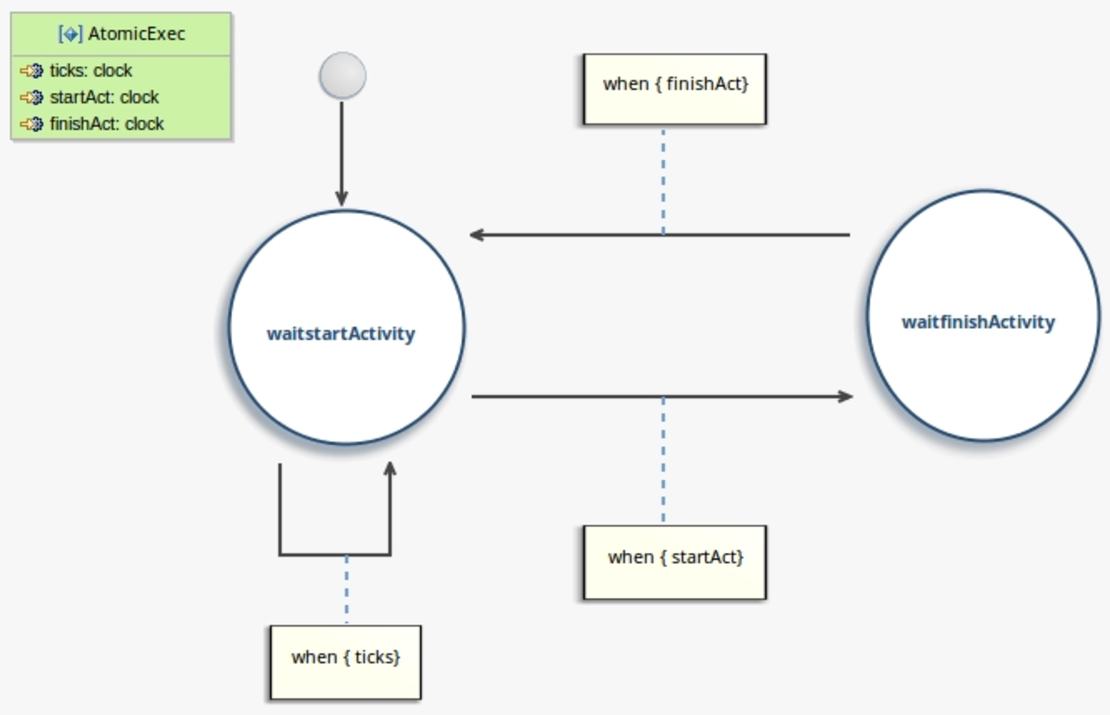
\includegraphics[width=.5\columnwidth]{examples/figs/AtomicExec}
		\label{fig:atomicexec}
	}
	\caption[]{State-based representation of the event relations in \moccml}
	\label{fig:subfigurestatebased}
\end{figure}


